In this section I'm going to first introduce what Protocol Buffers are.
Then, I'm going to analyze existing solutions of website documentations with the ability to call APIs for Protocol Buffers, GraphQL and RESTful APIs.
I'll start with Protocol Buffers, then I'll move and explore the solutions to GraphQL and finally I'll analyze RESTful API.


\section{Protocol Buffers}

\subsection{Types}

\subsection{Types}


\section{Website Documentation}

\subsection{Protocol Buffers}

\subsection{GraphQL}

\subsection{RESTful API}

\subsection{Summary}

\subsection{Issues}


\section{Requirements}
On the basis of the previously described problems and main requirements, I have compiled functional and non-functional requirements covering the required functionality of the static web generator.

\subsection{Functional}
% Co má systém umět

%\subsubsection{F1 -- Pomocník pro inicializaci obrazu softwaru Syllabus Plus}
%Pro inicializaci obrazu softwaru Syllabus Plus a další práci s daty je potřeba zadat informace o daném semestru.
%Správné nastavení je klíčové pro korektní plánování časových lístků.

\subsection{Non-Functional}

%\subsubsection{N1 -- Aplikace s grafickým uživatelským rozhraním}
%Aplikace by měla mít grafické uživatelské rozhraní pro práci s daty.
%Uživatel by tak měl být schopen obsluhovat aplikaci sám bez pomoci další osoby.


\section{Use Cases}


%\begin{figure}
%    \centering
%    \captionsetup{justification=centering}
%    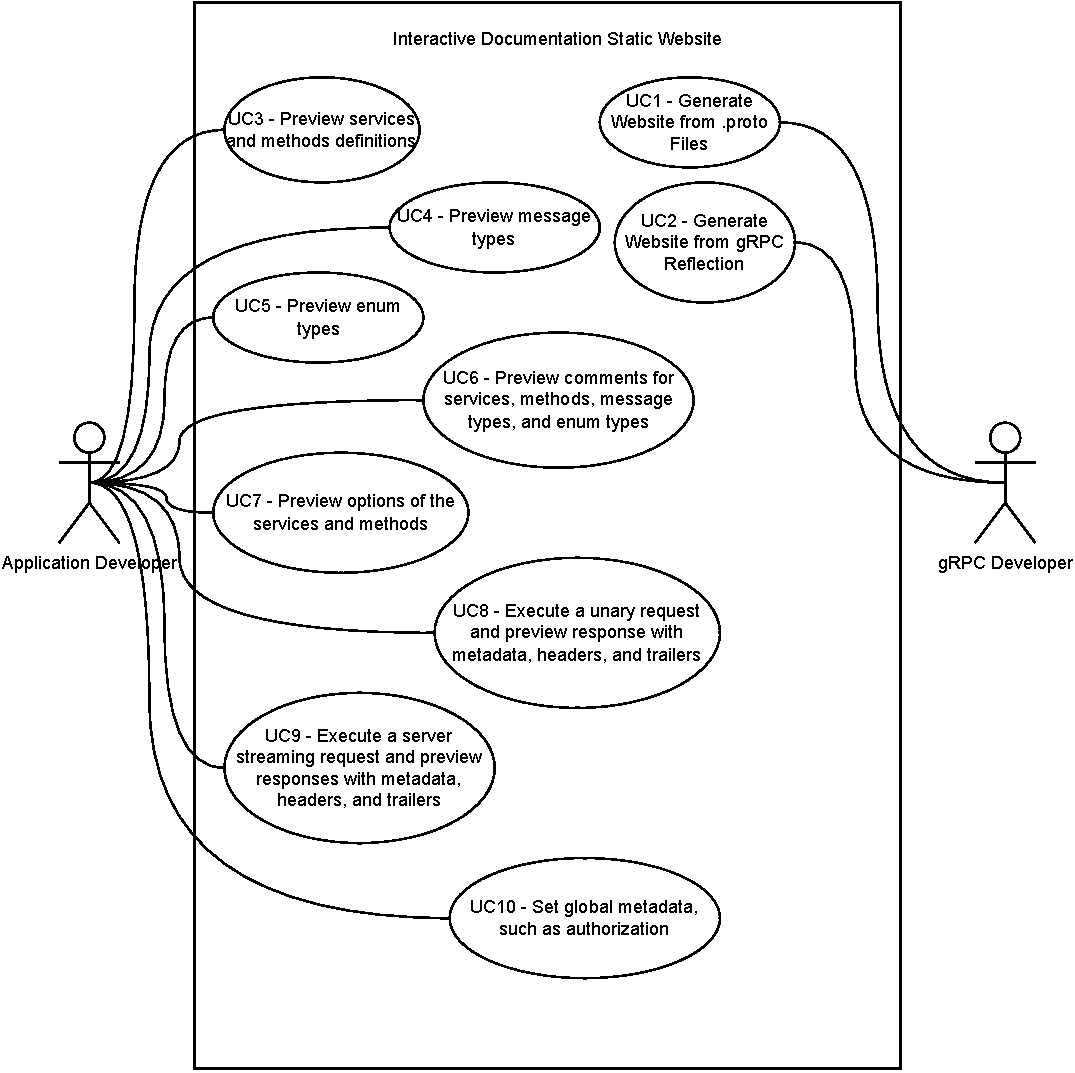
\includegraphics[width=1.0\textwidth]{use-case-diagram}
%    \caption{Diagram případů užití}
%    \label{fig:use-case-diagram}
%\end{figure}

%\subsection{UC1 -- Inicializace obrazu softwaru Syllabus Plus}
%Rozvrhář spustí software Syllabus Plus a začne s inicializací nového obrazu.
%Během inicializace se mu zobrazí dialog pro nastavení začátku semestru, vyučované dny, začátek a konec hodin, počet hodin za den a počet týdnů na semestr.
%Rozvrhář otevře aplikaci pro převod a nastaví semestr, který se využije pro načítání dat ze systému KOS\@.
%Zobrazí si jakým způsobem má položky nastavit, aby byla data správně reprezentována (například při plánování časových lístků).
%Formulář vyplní podle získaných dat z aplikace a inicializuje obraz.
%V případě, že se rozvrhář splete, musí aktuální obraz smazat a začít vytvářet nový od začátku.
%Jinak je inicializace úspěšně dokončena.


\section{Requirements to Use Cases Mapping}
I have compiled a table of requirements and use cases mapping (see table~\ref{tab:use_cases}) to verify that all requirements are covered by at least one use case and that no use case is unnecessary.
The table shows that all requirements are covered.

\begin{table}[hbt!]
    \centering
    \captionsetup{justification=centering}
    \begin{tabular}{|l|l|l|l|l|l|l|l|l|l|l|l|l|l|l|l|}
        \hline
        & \multicolumn{15}{c|}{Use Cases} \\ \hline
        & 1 & 2 & 3 & 4 & 5 & 6 & 7 & 8 & 9 & 10 & 11 & 12 & 13 & 14 & 15 \\ \hline
        F1  & x &   &   &   &   &   &   &   &   &    &    &    &    &    &    \\ \hline
        F2  &   &   & x &   &   &   &   &   &   &    &    &    &    &    &    \\ \hline
        F3  &   &   &   & x &   &   &   &   &   &    &    &    &    &    &    \\ \hline
        F4  &   &   &   &   &   &   &   &   &   &    &    &    &    &    & x  \\ \hline
        F5  &   &   &   &   & x &   &   &   &   &    &    &    &    &    &    \\ \hline
        F6  &   & x &   &   &   &   &   & x &   &    &    & x  & x  &    &    \\ \hline
        F7  &   & x &   &   &   &   &   &   &   &    &    & x  &    &    &    \\ \hline
        F8  &   &   &   &   &   &   &   &   &   &    &    &    & x  &    &    \\ \hline
        F9  &   & x &   &   &   &   &   &   &   &    & x  &    &    &    &    \\ \hline
        F10 &   & x &   &   &   &   &   &   &   &    &    &    &    &    &    \\ \hline
        F11 &   &   &   &   &   &   &   &   & x & x  &    &    &    &    &    \\ \hline
        F12 &   & x &   &   &   &   &   &   &   &    &    &    &    &    &    \\ \hline
        F13 &   &   &   &   &   &   &   &   &   & x  &    &    &    &    &    \\ \hline
        F14 &   &   &   &   &   &   &   & x & x & x  &    & x  & x  &    &    \\ \hline
        F15 &   &   &   &   &   &   &   & x & x & x  &    & x  &    &    &    \\ \hline
        F16 &   &   &   &   &   &   &   & x & x & x  &    & x  & x  &    &    \\ \hline
        F17 &   &   &   &   &   & x & x &   &   &    &    &    &    &    &    \\ \hline
        F18 &   &   &   &   &   & x &   &   &   & x  &    &    &    & x  &    \\ \hline
        F19 & x &   &   &   &   &   &   &   &   &    &    &    &    &    &    \\ \hline
    \end{tabular}
    \caption{Requirements to Use Cases Mapping}
    \label{tab:use_cases}
\end{table}